
\chapter{Getting Ready for a Biomedical Question Answering System}

In this task, you won't need to write any code (except that you need to edit
your Wiki page in Github flavored markdown language), instead you will learn a
new biomedical question answering task. Plus, we will also mention how to create
Milestones and Issues in the GitHub ISSUES system. Finally, you will create your
own question answering system based on an archetype framework called
\texttt{hellobioqa} we built for you.

We encourage you to go over the CSE Tutorial (which can be downloaded from the
blackboard) to know the baseqa framework for the question answering framework.
If you are still unsure how to create a repository on GitHub, or how to create a
Maven project from an archetype, we also recommend you to take a look at
Homework 0 and 1 again.


\section{Learning biomedical question answering task}

Question Answering (QA) is a computer science discipline within the fields of
information retrieval and natural language processing (NLP) which is concerned
with building systems that automatically answer questions posed by humans in a
natural
language.\footnote{\url{https://en.wikipedia.org/wiki/Question_answering}} The
system you are going to build will handle biomedical questions, e.g., ``What is
the role of PrnP in mad cow disease?''. As you can see, different from a generic
question answering, a biomedical QA system requires domain specific knowledge
bases, NLP tools, literature collections, etc., in order to answer such
questions.

One of the biomedical information retrieval benchmark is TREC Genomics
Task\footnote{\url{http://ir.ohsu.edu/genomics}}. The Text Retrieval Conference
(TREC) every year provides a platform for testing and experiments of retrieval
methods for different tasks. The Genomics Track for 2006 focuses on retrieval of
relevant passages within an article collection from biomedical journals as
answers to the questions in biomedical domain.

The genomics track provides 28 topics (or questions)\footnote{Strictly, a topic
is an information need, that can be expressed literally differently as many
different questions, but here we use topic and question interchangably.} created
by active biological researchers. Each topic fit within one of four
question-oriented topic templates: the role of a gene in a disease, the effect
of a gene on a biological process, how genes interact in organ function, and how
mutations in genes influence biological processes. All the questions are listed
in Table \ref{tab:question}:

\begin{table}[t] \centering
\caption{28 topics (or questions) from TREC Genomics 2006\label{tab:question}}
\small
\begin{tabular}{lp{32em}}
\hline
ID & Question \\
\hline
160 & What is the role of PrnP in mad cow disease? \\
161 & What is the role of IDE in Alzheimer's disease \\
162 & What is the role of MMS2 in cancer? \\
163 & What is the role of APC (adenomatous polyposis coli) in colon cancer? \\
164 & What is the role of Nurr-77 in Parkinson's disease? \\
165 & How do Cathepsin D (CTSD) and apolipoprotein E (ApoE) interactions contribute to Alzheimer's disease? \\
166 & What is the role of Transforming growth factor-beta1 (TGF-beta1) in cerebral amyloid angiopathy (CAA)? \\
167 & How does nucleoside diphosphate kinase (NM23) contribute to tumor progression? \\
168 & How does BARD1 regulate BRCA1 activity? \\
169 & How does APC (adenomatous polyposis coli) protein affect actin assembly \\
170 & How does COP2 contribute to CFTR export from the endoplasmic reticulum? \\
171 & How does Nurr-77 delete T cells before they migrate to the spleen or lymph nodes and how does this impact autoimmunity? \\
172 & How does p53 affect apoptosis? \\
173 & How do alpha7 nicotinic receptor subunits affect ethanol metabolism? \\
174 & How does BRCA1 ubiquitinating activity contribute to cancer? \\
175 & How does L2 interact with L1 to form HPV11 viral capsids? \\
176 & How does Sec61-mediated CFTR degradation contribute to cystic fibrosis? \\
177 & How do Bop-Pes interactions affect cell growth? \\
178 & How do interactions between insulin-like GFs and the insulin receptor affect skin biology? \\
179 & How do interactions between HNF4 and COUP-TF1 suppress liver function? \\
180 & How do Ret-GDNF interactions affect liver development? \\
181 & How do mutations in the Huntingtin gene affect Huntington's disease? \\
182 & How do  mutations in Sonic Hedgehog genes affect developmental disorders? \\
183 & How do  mutations in the NM23 gene affect tracheal development? \\
184 & How do  mutations in the Pes gene affect cell growth? \\
185 & How do  mutations in the hypocretin receptor 2 gene affect narcolepsy? \\
186 & How do  mutations in the Presenilin-1 gene affect Alzheimer's disease? \\
187 & How do  mutations in familial hemiplegic migraine type 1 (FHM1) gene affect calcium ion influx in hippocampal neurons? \\
\hline
\end{tabular}
\end{table}

Documents for this task come from a corpus of 162,048 full-text biomedical
articles. If you want to estimate the size of the corpus, 12.3 GB (uncompressed)
and 3 GB (standard compressed). Each document is identified by its PMID
(PubMed\footnote{\url{http://www.ncbi.nlm.nih.gov/pubmed}} ID). Postprocessing
is done to eliminate as much non-article material as we could from the original
HTML formats Legal spans are defined as any text > 0 bytes in length between an
HTML paragraph tag, which is any tag that starts with \verb|<p| or \verb|</p|.

Similar to what you will be asked by the BioCreative competition organizer, you
are required to follow an output format for the retrieved relevant passages. The
format for TREC Genomics complies with standard TREC output format: a tabular
format that consists seven fields: topic number, doc ID (PubMedID), rank, score,
passage start, passage length, run tag.

The evaluation for the relevant passage retrieval is measured with a variant of
mean average precision (MAP). Three different levels will be applied to the
final result:
passage-level, document-level and aspect-level. In addition to the passage-level
evaluation, document-level captures the coverage of different relevant
documents, and aspect-level evaluation captures the coverage of different MeSH
terms\footnote{\url{http://www.ncbi.nlm.nih.gov/mesh}}.

\subsection{HelloBioQA: BioQA framework and testbed implementation}

We will briefly describe how the HelloBioQA framework based on CSE can help
build your own QA pipeline, and evaluate your components automatically.

The input file ``trecgen06.txt'' has been put into the
\texttt{src/main/resources/input} directory, while consists of all the
questions, one per line. Each sentence will be preceded on the same line by a
sentence identifier, i.e.,

\begin{verbatim}
160|What is the role of PrnP in mad cow disease?
\end{verbatim}

The gold-standard relevant passages have also been included in HelloBioQA
framework (\texttt{src/main/resources/gs/trecgen06.passage}) project, in
addition, we manually annotated keyterms for the questions. Different from
homework 1, the character offsets DO consider whitespaces, which is adopted by
the UIMA framework. The gold-standard keyterms include not only the named
entities, but also other important key verbs. Although gold-standard keyterm
does not perfectly fit the requirement of NER evaluation, it will be used to
test your NER components (\texttt{src/main/resources/gs/trecgen06.keyterm}). We
won't consider the evaluation result in M1 when grading your homework.

We have implemented everything you need for collection reader, gold standard
decorator, and evaluators, which means you don't need to put any effort to
investigate how to read the questions and generate the output format in this
homework. But we still encourage you to investigate how three different levels
of MAP evaluation work. At the end of your pipeline execution, you will see the
evaluation results similar to the following:

\small
\begin{verbatim}
 ------------------ EVALUATION REPORT ------------------
Experiment: ac146544-b116-4cce-897e-77bfa1b4fc18:1
Evaluator,Configuration,Precision,Recall,F-1,MAP,Binary Recall,Count
RetrievalMeasuresEvaluator,1|SimpleKeytermExtractor[persistence-provi
der:inherit: ecd.default-log-persistence-provider]>2|SimpleSolrRetrie
valStrategist[hit-list-size:10#embedded:true#core:data/guten#persiste
nce-provider:inherit: ecd.default-log-persistence-provider ]>3|Simple
PassageExtractor[hit-list-size:10#embedded:true#core:data/guten#keyte
rmWindowScorer:edu.cmu.lti.oaqa.openqa.hello.passage.KeytermWindowSco
rerSum#persistence-provider:inherit: ecd.default-log-persistence-prov
ider],0.5000,0.6667,0.5714,0.6667,1.0000,1

 -------------------------------------------------------
 ------------------ EVALUATION REPORT ------------------
Experiment: ac146544-b116-4cce-897e-77bfa1b4fc18:1
Evaluator,Configuration,Precision,Recall,F-1,MAP,Binary Recall,Count
RetrievalMeasuresEvaluator,1|SimpleKeytermExtractor[persistence-provi
der:inherit: ecd.default-log-persistence-provider]>2|SimpleSolrRetrie
valStrategist[hit-list-size:10#embedded:true#core:data/guten#persiste
nce-provider:inherit: ecd.default-log-persistence-provider ]>3|Simple
PassageExtractor[hit-list-size:10#embedded:true#core:data/guten#keyte
rmWindowScorer:edu.cmu.lti.oaqa.openqa.hello.passage.KeytermWindowSco
rerSum#persistence-provider:inherit: ecd.default-log-persistence-prov
ider],0.2000,0.3333,0.2500,0.3056,1.0000,1

 -------------------------------------------------------
 ------------------ EVALUATION REPORT ------------------
Experiment: ac146544-b116-4cce-897e-77bfa1b4fc18:1
Evaluator,Configuration,DocumentMAP,PassageMAP,AspectMAP,Count
PassageMAPMeasuresEvaluator,1|SimpleKeytermExtractor[persistence-prov
ider:inherit: ecd.default-log-persistence-provider]>2|SimpleSolrRetri
evalStrategist[hit-list-size:10#embedded:true#core:data/guten#persist
ence-provider:inherit: ecd.default-log-persistence-provider ]>3|Simpl
ePassageExtractor[hit-list-size:10#embedded:true#core:data/guten#keyt
ermWindowScorer:edu.cmu.lti.oaqa.openqa.hello.passage.KeytermWindowSc
orerSum#persistence-provider:inherit: ecd.default-log-persistence-pro
vider],0.3056,0.0202,1.0000,1 
\end{verbatim}
\normalsize

Three big tables correspond to the evaluation at different phases, the first
table is the result for keyterm extraction, and the sencond table for relevant
document retrieval, and the last table is for the final passage extraction. If
you have more than traces running (e.g., multiple options for NER), then you
will see multiple lines for each of the traces. If you are familiar with
information retrieval, then the evaluation for keyterm extraction and document
retrieval follows the standard definitions for Precision/Recall/F-1/MAP/etc., if
you are unfamiliar, we suggest you to search them in Wikipedia or other
information retrieval textbooks. Believe me, all of them are easy to understand!
The evaluation for passage extraction follows a variant of MAP definition, you
can find detailed algorithm from the task's homepage.

% move them to task 2?
What you need to implement is only the \verb|pipeline| (if you are wondering why
I am using typewriter font for ``pipeline''. please take a look at the CSE
Tutorial again). The pipeline will consist of three major phrases, which have
been defined in BaseQA framework. (If you couldn't remember what they are, I
again encourage you to go over the CSE Tutorial.) In fact, you can define
totally different phrases and put them into your QA pipeline\footnote{For
example, Statistical Source Expansion for Question Answering,
\url{http://dl.acm.org/citation.cfm?id=2063632}}, but for this task, you are
recommended to focus on this ``traditional'' pipeline design, so that we can
easily bundle your components for the big experiment.

Before you think about the architecture and engineering, it's a good time to
have a discussion among the team members and talk about what you can do to
improve the performance based on the baseline implementation given by the
HelloQA project. Put them in your Wiki page, and in the next subtask, you will
learn how to create the Wiki.

\begin{qa}

\item[Q1] I've looked into the baseline implementations in HelloQA. Can you give
us some more ideas on how to improve the system?

\item[A1] Actually, since it is a past TREC task, you can easily find the papers
from participants that describe how they tackled it. Another paper you might be
interested in is the task overview paper from the organizer. They summarized
many algorithms, and knowledge sources, when the competition was over:
\url{http://trec.nist.gov/pubs/trec15/papers/GEO06.OVERVIEW.pdf}.

\item[Q2] Where is the type system for HelloBioQA?

\item[A2] As type system is a task specific, you should look for the one called
\texttt{OAQATypes.xml} in \texttt{BaseQA}.

\end{qa}



\section{Team coding with GitHub}

You will again use GitHub to host your project code. But different from previous
homeworks, all the team members need to collaborate on the project, and commit
the code changes to the same repository, which means it is good to learn how to
more about git and GitHub in this subtask.

\subsection{Creating a repository}

\begin{enumerate}

\item The team leader needs to create a repository with his/her GitHub acccount,
and name your project as \texttt{hw2-teamXX}, where \texttt{XX} is your team
number, which is a two-digit number ranging from 01 to 18. If you are not sure
how to create a GitHub repository, please refer to Homework 0.

At this point, all the team members are able to checkout the empty project and
start working on their own. But this is NOT recommended! We recommend the team
leader could checkout the project from GitHub repository, go through the entire
Maven project building process (we will come to this in the next subtask) until
you can ran a simple hellobioqa pipeline. Then, the team leader again, from
his/her laptop, commits and pushes everything to the repository before the team
members clone the project.

\item Now, everyone has the read permission to your project repository (since it
is a public repository). To help your team members gain read/write permissions,
you, the team leader, should add them as collaborators. You need to click the
\textbf{Admin} tab on your project homepage, and click the
\textbf{Collaborators} menu on the left. Put in your teammates' GitHub IDs one
by one, and click \textbf{Add} button.

\end{enumerate}

\subsection{Creating milestones, issues, and Wiki pages}

To create milestones for your development will help better organize your team
members, know your collaborators' progress, and help users/customers know what
they could expect from a future release. Issues can be detailed action items
team members would like to contribute to each milestone. Action can be bug fix,
feature enhancement, etc. If you are still unclear what a milestone is or what
an issue is, or you want to understand how milestone and issue tracking system
can help software development, you can search on Google and find out many
interesting blogs. You are recommended to read about the features of GitHub
issue tracking system at
\url{https://github.com/blog/831-issues-2-0-the-next-generation} and
\url{https://github.com/features/projects/issues}.

We recommend all the team members have a discussion on how to set the
milestones, and what your first several initial issues will be (i.e., what they
first couple of things you want to do at the beginning.) And the team leader
does the following steps. \textbf{Remember that you are unlikely to submit all
the issues to the tracking system at once, you may create new issues for bugs to
fix or new features to implement, change the owner (assignee) of the issue,
close implemented issues, or mark some as wontfix. All your team members
are responsible to maintain your milestones and issues.}

\begin{enumerate}

\item To create a milestone, you can navigate to the \textbf{Issues} tab of your
project homepage, then click the \textbf{Milestones} below the main menu bar.
Now you are able to see the button \textbf{Create a new milestone}, click it.

\item Type your title for the milestone, e.g., ``M1'' for the first milestone
(you can also make it more meaningful and specific). Write a few descriptions
for this milestone, like the goal and the brief descriptions of features will be
enhanced in this milestone. Finally, select a ``Due Data'' for the milestone.
Click the ``Create Milestone'' to finalize creating your milestone.

\item Do the previous step once again until all your milestones are created.

\item Now, you need to submit your first several issues. Go back to the
\textbf{Issues} tab on your project homepage, and click \textbf{New Issue}. Type
a title, assign the task to a particular team member, link this issue to a
previously created milestone. Finally write down detailed comments to the issue.

You may find when you type ``@'' followed by your collaborator's ID in the
comment box, you are able to mention your collaborator as you mention your
friend in a tweet on Twitter.

You can learn how to write in GitHub Flavored Markdown language, by clicking the
link above the textbox.

You can also attch labels to each issue by selecting them from the right panel.
As we mentioned earlier, you can change the milestone assignment, in particular,
if you find you couldn't finish it by M1, then you can change it to M2 later, or
you can also relabel it as \textbf{wontfix}.

\end{enumerate}

Now, you can create a Wiki page for your team meeting minutes and other
important items.

\begin{enumerate}

\item Click the ``Wiki'' tab at the top of your project homepage, and click
\textbf{Edit Page} to start editing it.

\end{enumerate}

Once you reach this point, remember to send us an email to report the URL of
your project repository page (e.g., \url{https://github.com/ID/hw2-teamXX}).

\subsection{Team coding with git-branch, git-merge, git-rebase}

Collaboration is important for this homework. All the team members start their
individual development after the team leader gets the framework ready, and
pushes all his/her local commits to the repository. Once a team member finalizes
his/her development, he/she might take responsibility on another task, or want
to check the integrity or compatibility with features implemented by
collaborators. After all the individual developments are done, team leader is
responsible to merge all the newly developed components into the same codebase
and test the integrity.

Git branching is a good tool to help the team manage parallel development and
distributed codebase. In fact, the branching mechanism is widely adopted by not
only git, but many other version control systems, e.g., SVN or Mercurial (Hg).
But one of the most important reasons that people love git branching over SVN or
Mercurial (Hg) is its light-weight nature, which allow switching between
development branches within the same clone of a repository.

Normally, the team leader is in charge of the \texttt{master} branch (the one
you probably used for homework 0 and 1), which usually corresponds to a codebase
for the most recent stable release, while team members should create branches
for each individual task assignment, e.g., bug fixes, feature enhancement with
\texttt{git branch} command. You can also do it within Eclipse by right-clicking
the project name, and select \textbf{Team} $\rightarrow$ \textbf{Switch To}
$\rightarrow$ \textbf{New Branch\ldots}.

To merge multiple development branches back to \texttt{master} branch (or in
Eclipse \textbf{Team} $\rightarrow$ \textbf{Switch To} $\rightarrow$
\textbf{master}), you should switch back to master, and then \texttt{git merge}
the branch you want to be merged (or \textbf{Team} $\rightarrow$
\textbf{Merge\ldots}). Sometimes, you may also need \texttt{git rebase} when you
later realize your development should depend on another feature that was also
being developed by your collaborator, which hadn't beed integrated in the
\texttt{master} branch by the time you created your development branch.

To better understand git branching, you should read the ``Git Branching''
chapter of Pro Git Book (\url{http://git-scm.com/book/en/Git-Branching}). You
can also find a more sophisticated branching model at
\url{http://nvie.com/posts/a-successful-git-branching-model/}, which may be too
complicated for this homework, but it can inspire how you want to manage your
branches.

If you are looking for a Eclipse plug-in that can bring the GitHub issue
tracking system to your workspace, e.g., create/close/comment issues, label
them, assign to a person within eclipse, or automatically get notified by a
message bubble if an issue is assigned to you, then you can try to investigate
Mylyn plug-in. In the ``Tips and Tricks using Eclipse with Github''
post\footnote{
\url{http://eclipsesource.com/blogs/2012/08/28/tips-and-tricks-using-eclipse-with-github/}}
, you will find the basic idea how Mylyn GitHub connector works. By default,
Eclipse Juno for Java developers comes with EGit, Mylyn, and Mylyn Github
connector, and the Task View is on the top-right corner of the Java perspective
by default.



\section{Performing a Maven Release}

In the last task, you will need to submit your Java code by performing a release
of your code. But remember that Maven release plug-in will check if all the
changes you have made have been checked into the remote repository (i.e. GitHub
in our case). So, let's perform a git-commit and a git-push.

\begin{enumerate}

\begin{figure}
\hspace{-1em}
\begin{minipage}{0.5\textwidth}
\centering
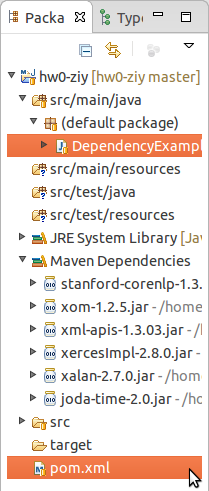
\includegraphics[scale=0.3]{simple-code-05-commit}
\caption{Performing a git-commit/push before preparing a release\label{simple-code-05-commit}}
\end{minipage}
\hfill
\begin{minipage}{0.5\textwidth}
\centering
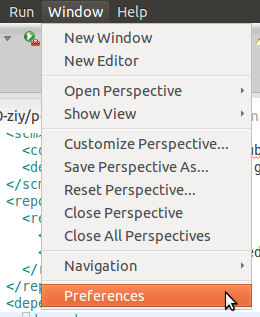
\includegraphics[scale=0.3]{submit-01-preference}
\caption{Starting to add an external Maven executable\label{submit-01-preference}}
\end{minipage}
\hspace{-1em}
\end{figure}

\item Similar to what you did earlier, you execute git-commit and git-push to
the project, and you could see the ``greater than'' symbol disappears and a
``master'' label is attached to project path, which means you are successful
with your git-commit and git-push.

\begin{figure}
\hspace{-2em}
\begin{minipage}{0.5\textwidth}
\centering
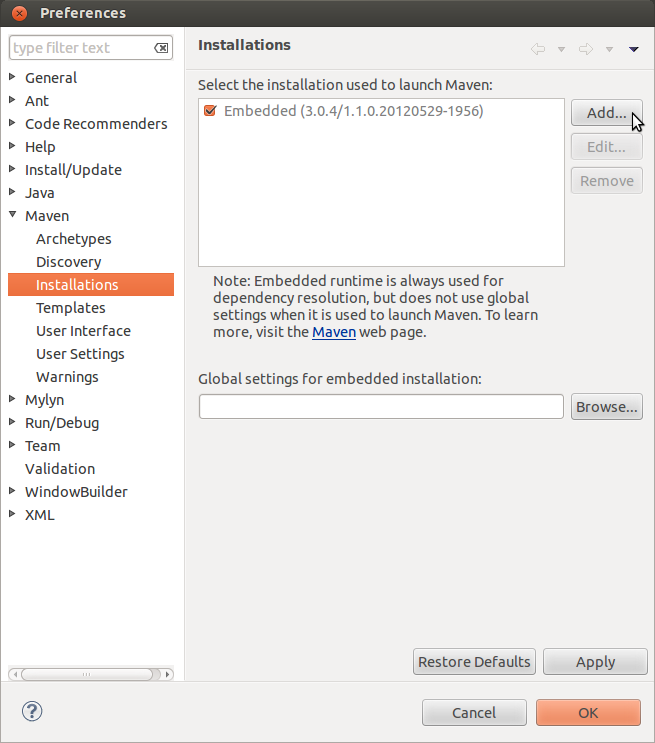
\includegraphics[scale=0.3]{submit-02-add-maven}
\caption{Adding another Maven executable\label{submit-02-add-maven}}
\end{minipage}
\hfill
\begin{minipage}{0.5\textwidth}
\centering
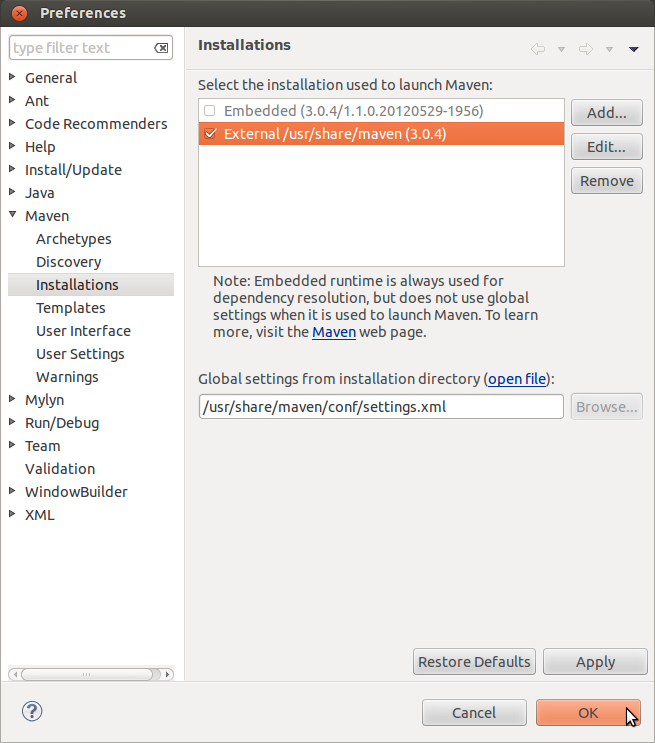
\includegraphics[scale=0.3]{submit-03-add-maven-done}
\caption{Viewing the added external Maven\label{submit-03-add-maven-done}}
\end{minipage}
\hspace{-2em}
\end{figure}

\item Sometimes, the embedded Maven runtime from m2e cannot be succesfully
executed to perform a release goal. Therefore, we should add the externally
installed Maven runtime into the Eclipse. Click \textbf{Window} (or
\textbf{Edit}) $\rightarrow$ \textbf{Preferences} (see Figure
\ref{submit-03-add-maven-done}).

\item Select \textbf{Maven} $\rightarrow$ \textbf{Installations}. You will see
the ``Embedded'' runtime (as shown in Figure \ref{submit-02-add-maven}). Click
\textbf{Add\ldots} to locate the installation path of your Maven runtime.

\item Then, you could see an ``External'' runtime in the installation lists. See
Figure \ref{submit-03-add-maven-done}.

\begin{figure}
\centering
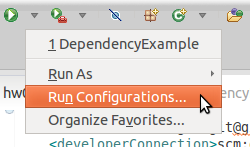
\includegraphics[scale=0.3]{submit-04-run-config}
\caption{Getting ready for a release\label{submit-04-run-config}}
\end{figure}

\item Now you can execute a Maven goal within Eclipse (of course, you can also
do that outside Eclipse from command line). Click the down-arrow next to the
\textbf{Run} button, and select \textbf{Run Configurations\ldots}. See Figure
\ref{submit-04-run-config}.

\begin{figure}
\centering
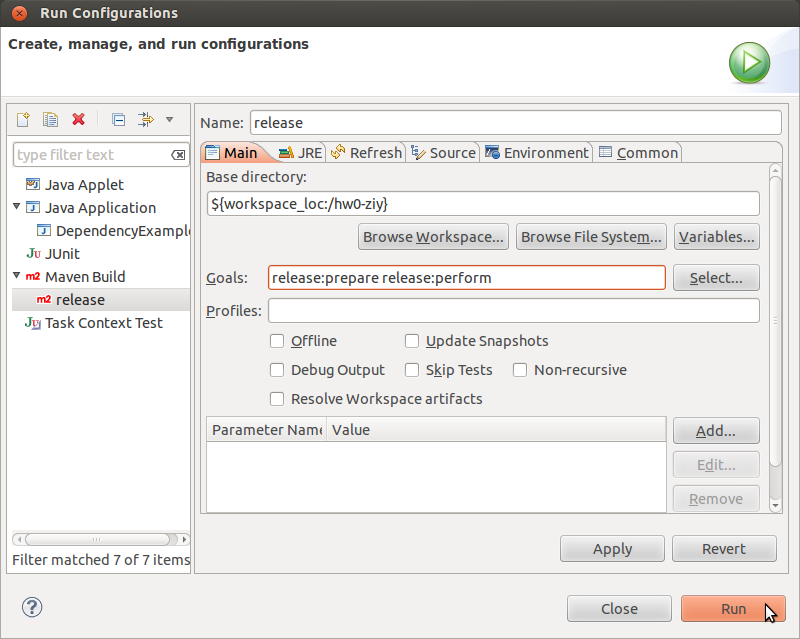
\includegraphics[scale=0.3]{submit-05-run-config-done}
\caption{Configuring Maven goal\label{submit-05-run-config-done}}
\end{figure}

\item In the ``Run Configurations'' window, double-click \textbf{Maven Build} to
create a new Maven goal. See Figure \ref{submit-05-run-config-done}. Rename your
run configuration name as ``release'' (optional), and click \textbf{Browse
Workspace\ldots} to select your project, and type in your goals as follows:

\begin{verbatim}
release:prepare release:perform
\end{verbatim}

This actually defines two goals ``release:prepare'' and ``release:perform''. As
you will probably encounter tons of errors during this step, we should review
some details of the Maven release.

The Maven
guide\footnote{\url{https://maven.apache.org/guides/mini/guide-releasing.html}}
tells us what is happening behind these two goals:

\begin{quote}
The release:prepare goal will:

\begin{enumerate}
\item Verify that there are no uncommitted changes in the workspace.
\item Prompt the user for the desired tag, release and development version
names.
\item Modify and commit release information into the pom.xml file.
\item Tag the entire project source tree with the new tag name.
\end{enumerate}

The release:perform goal will:

\begin{enumerate}
\item Extract file revisions versioned under the new tag name.
\item Execute the maven build lifecycle on the extracted instance of the
project.
\item Deploy the versioned artifacts to appropriate local and remote
repositories.
\end{enumerate}
\end{quote}

If the goals are not executed sucessfully, a relatively useful message will be
printed out to console to help you discover where the problem is.

\begin{figure}
\centering
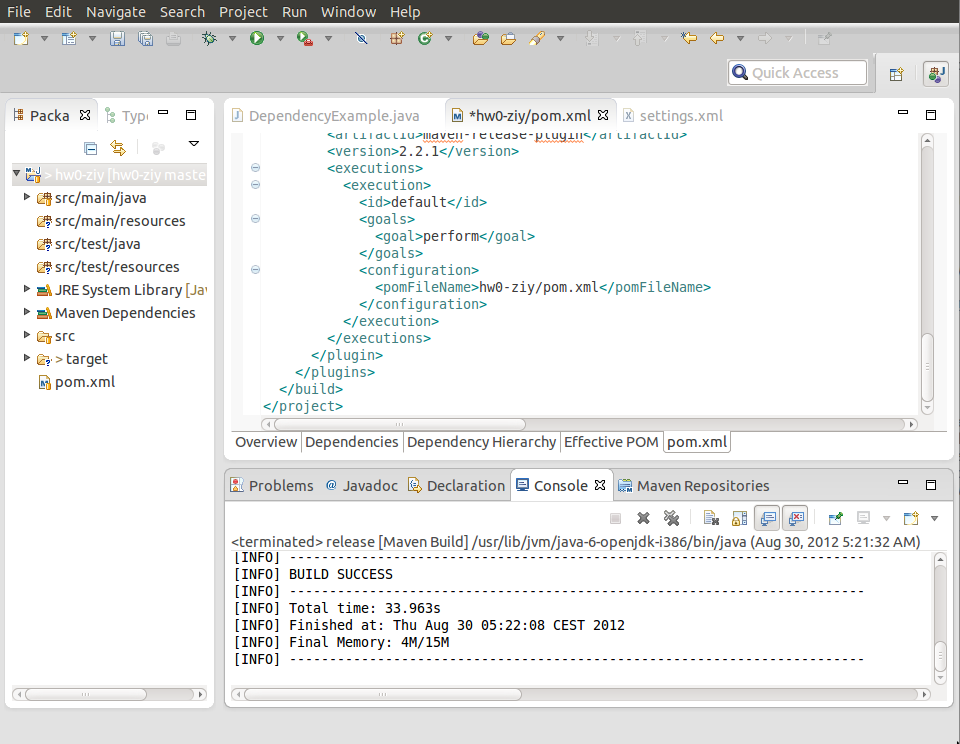
\includegraphics[scale=0.3]{submit-06-release}
\caption{A successful release!\label{submit-06-release}}
\end{figure}

\item Finally after you fixed all the problems (if any), you could see the very
pleasant ``BUILD SUCCESS'' message in the console (as shown in Figure
\ref{submit-06-release}), which means you've done with your Homework 0!
Congratulations!

\begin{qa}

\item[Q1] The ``release:prepare'' goal could be executed successfully, but there
was an error during ``release:perform''. How can I start all over
again?\footnote{Reported by Kartik Mandaville.}

\item[A1] A successful ``prepare'' with an unsuccessful ``perform'' always leads
to a very subtle situation. Sometimes, you can try to execute a
``release:rollback'' Maven goal to revert to the previous status, or you are try
to manually delete the \verb|release.properties| file under your project
diretory, and make sure you are now working on a SNAPSHOT version. (You can
check your version from Maven POM Editor, and you have an opened Maven POM
Editor, be sure to close it and open it again since it will not be automatically
refreshed after you execute a Maven goal.) If it is no longer a SNAPSHOT
version, you should modify the \textbf{Version} field to something like
``0.0.2-SNAPSHOT'' (without quotes). You might want to refer to
\url{http://maven.apache.org/guides/mini/guide-releasing.html} about the details
of the release process.

\item[Q2] The process hangs forever during Maven ``release:prepare'' executing a
``git push'' command, in other words, it doesn't terminate or produce any
further useful information. What should I do?

\item[A2] We are sure there is some bug with the plugin related to this issue.
But there still some workarounds to consider.

\begin{enumerate}
\item If you generate a public key with a passphrase (i.e., you typed in
something before you pressed \textbf{Enter}), then try to regenerate another
public key following the same instruction and paste it to GitHub.
\item Try to log back into GitHub to see if your email address has been
verified.
\item Turn to command line to execute Maven goal by typing
\verb|mvn release:prepare release:perform| from the project directory to see
if it terminates automatically or still hangs there forever.
\item Try to find the last command in the log message shown in the console
(e.g., \verb|git push ... master:master|), and directly type in the same command
in the command line to see if additional verification (e.g., adding a host to
\verb|known_host| list) is required.
\end{enumerate}

\item[Q3] What if I find some bugs after it has been released? How can I
resubmit my code?

\item[A3] You can look at the ``Overview'' tab in the Maven POM Editor for your
pom.xml file. The version should be ``0.0.2-SNAPSHOT'', which indicates a
previous version has been generated. Now, you could redo this task (git-commit,
git-push, run Maven goals) to release the version 0.0.2. We will evaluate your
code based on the latest release.

\item[Q4] How could I check if my submission is successful?

\item[A4] First of all, don't worry about it, even if by the deadline, we
haven't received your submission, we will notify you, and help you check what
the problem may be before you start Homework 1.

If you want to check your submission, you can go to
\url{http://mu.lti.cs.cmu.edu:8081/nexus/index.html} back again, and log in with
your password, go to \textbf{View/Repositories} $\rightarrow$
\textbf{Repositories} on the left, then click \textbf{Course Releases} on the
right, unfold directories along the groupId path, and if you see your artifact
at the end, then you've done!

\end{qa}

\end{enumerate}
